\chapter{Quality of Experience}\label{chap:02}
\begin{chapter-abstract}
Here I give an overview on the concept of \ac{QoE}.
This is basically Psychophysics (Perception): Blauert, Möller, Jekosch and Raake.
I present standard assessment methods (\ac{ACR}, \ac{MUSHRA} etc.)and the underlying/implicit assumption for user studies).
However, the main focus on \textit{higher level} concepts (Moeller, ARCU and Geerts), which propose a more holistic approach towards \ac{QoE} and consider time and repeated usage.
At the end I will discuss, how QoE relates to concepts of Utility, Acceptability, Satisfaction and Service Quality (needed in chap 4).
Those concept are important from the business perspective.

I should here include also some technical examples why \ac{QoE} is important for \ac{IP}-based networks.
Specialized methods for assessment of temporal effects / performance fluctuations are presented in Chapter~\ref{chap:04}.
\end{chapter-abstract}


\section{Perception and Psychophysics}
%\item What is perception?
%\item What is psychophysics? Where does it come from?
Human use their senses, \ie perceptual organs, to perceive the events of their environment.
Based upon perceived events an internal model is created and updated, which incorporates knowledge about the environment and thus reality.
This model is then used to plan actions and updated, when new information including perceptual events are processed.
%\cite[p. 4]{blauert_spatial_1996}: "Auditory events, at first relatively diffuse in their locatedness, become more precisely defined spatially; the correspondence to the visual world and to other senses also become more precise."

%\item Perceptual Event (with Sensory Processing [QoE Book Chap 2]): A physical event may(!) trigger a
%\item (Physical) Event: An observable occurrence with time, location, character [Whitepaper] -> Duration? [me]
A \emph{perceptual event} occurs in a human observer occurs, when a \emph{physical event} stimulates a  sensory organ.
A physical event is an observable occurrence in time, location and character~\cite{callet_qualinet_2013}.
One example of a physical event is a sound event that reaches the ear results in an auditory event in the observer (see ~\ref{img:chap02:auditory-event}).
Because the perceptual event occurs in only in the observer, it cannot be observed directly.
Such an perceptual event can be described by the observer. %or series
This description can be done with quantitative or qualitative way.

\begin{figure}
%	\includegraphics[width=1\textwidth]{•}
	\caption{Perceptual event (Blauert stuff)}
	\label{img:chap02:auditory-event}
\end{figure}

%Just noticable difference

%\item Behavioral impact of perceptual events: anticipation and matching and exploratory actions [QoE Book Chap 2]

%\item Inherent assumption: perception is more or less reproducible: humans perceive similar

%\item Experience: An experience is an individual's stream of perception and interpretation of one or multiple events [Whitepaper].

%\item Definition of physical observable things may lead to perception AND may be memorized.

%\item What is experiencing? (cite book)
\begin{definition}[Experiencing]
``is the individual stream of perceptions (of feelings, sensory percepts and concepts) that occurs in a particular situation of reference.''~\citep[p. 13]{moller_quality_2014}.
\end{definition}

\section{Perceptual Quality}
\begin{itemize}
\item (Perceptual) Quality: Individual comparison and judgment process with perception, reflection (optional?) and description of the outcome (optional?) [whitepaper]
\item Quality formation process
\item Assumed quality + recalled quality
\item Expectations: Prior experiences, Desired nature, Internal reference, Contextual Factors, Task [Moeller, Raake] 
\item Perceptual Quality Features, Quality Elements, Perceptual dimensions [Moeller, Raake]%NOTE: Features only very short!
%NOPE \item Semiotic triangle [Raake, Buch p.2]: sign carrier, referent and meaning; (is similar to Shannon)
\item What are related concepts: QoS, Performance?
\item Check Geerts for broader context!
\item Moeller DISS taxonomy
\item REF Gaming taxonomy, if used later!
\item Lab vs. field studies
\end{itemize}

\begin{figure}
	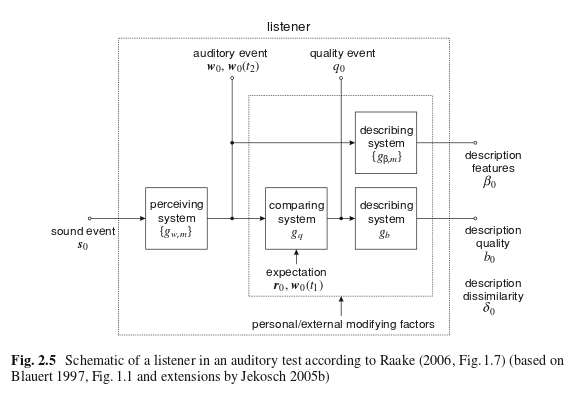
\includegraphics[width=1\textwidth]{fig/quality-event}
	\caption{Quality event}
	\label{img:chap02:quality-event}
\end{figure}


\begin{definition}[\acf{QoE}]
``is the degree of delight or annoyance of a person whose experiencing involves an application, service, or system. It results from the person’s evaluation of the fulfillment of his or her expectations and needs with respect to the utility and / or enjoyment in the light of the person’s context, personality and current state.''~\citep[p. 21]{moller_quality_2014}.
\end{definition}

\begin{definition}[Assumed quality]
``corresponds to the quality and quality features that users, developers, manufacturers or  service  providers assume regarding a  system, service or product that they intend to be using, or will be producing, without however grounding these assumptions on an explicit assessment of \textit{quality based on experiencing}.''~\citep[p. 20]{moller_quality_2014}.
\end{definition}


\begin{figure}
	
\includegraphics[width=1\textwidth]{fig/quality7pt_scale}
	\caption{Continuous 7-point scale for \ac{ACR} with German labels; labels from left-to-right: extremely bad (0), bad (1), poor (2), fair (3), good (4), excellent (5) and ideal (6) \citep{itu-t_p.805:_2007}.}
	\label{img:chap02:qualityScale}
\end{figure}

\section{Application of Quality of Experience}
\begin{itemize}
\item How is this studied? How is QoE typically assessed? (Methods)? 
\item Practical outcome? Evaluation procedures, knowledge and Objective Models (for different purpose)

\item Approaches towards modeling: how to one create a model? What are limitations?
\item Types of judgment: momentary and retrospective
\item Performance fluctuations: temporal effects; outlook to next chapter.
\item Where degradations come from? (production/recording, coding, transmission, reproduction)
\item \cite{pitrey_aligning_2011}
\item Minker/Weiss Book
\end{itemize}


\section{Related concepts}
\begin{itemize}
\item Definition of Utility [Kahneman and also Moeller]
\item Definition of Acceptability with regard to Service
\item Definition of Satisfaction (if required?)
\item Service quality
\end{itemize}
